\documentclass[11pt,a4paper]{article}

\usepackage[utf8]{inputenc}
\usepackage[spanish]{babel}
\usepackage[T1]{fontenc}
\usepackage[margin=2.5cm]{geometry}
\usepackage{graphicx}
\usepackage{xcolor}
\usepackage{listings}
\usepackage{hyperref}
\usepackage{enumitem}
\usepackage{fancyhdr}
\usepackage{booktabs}

\definecolor{codebg}{RGB}{245,245,245}
\definecolor{codekw}{RGB}{0,90,150}

\lstdefinestyle{docker}{
  backgroundcolor=\color{codebg},
  basicstyle=\ttfamily\small,
  keywordstyle=\color{codekw}\bfseries,
  commentstyle=\color{gray},
  showstringspaces=false,
  breaklines=true,
  frame=single,
  numbers=left,
  numberstyle=\tiny\color{gray},
  morekeywords={FROM,COPY,EXPOSE,RUN,CMD,ENTRYPOINT,WORKDIR}
}

\lstdefinestyle{shell}{
  backgroundcolor=\color{codebg},
  basicstyle=\ttfamily\small,
  showstringspaces=false,
  breaklines=true,
  frame=single
}

\pagestyle{fancy}
\fancyhf{}
\rhead{Cloud Computing}
\lhead{Laboratorio 2}
\rfoot{\thepage}

\title{Laboratorio 2: Containerización de un Servidor Web}
\author{Diego Raúl Rivas Huanca \\ Grupo de laboratorio: \_\_\_ \\ \textit{(completar con el grupo real)}}
\date{\today}

\begin{document}

\maketitle

\section{Objetivo}
Investigar y construir una imagen de contenedor que permita ejecutar un
servidor web, comprendiendo la relación entre la aplicación, la
imagen, el contenedor y los puertos del contenedor y de la máquina
virtual.

\section{Situación}
Una aplicación web debe ejecutarse dentro de un contenedor. Se
construyó una imagen mediante un \texttt{Dockerfile}, se ejecutó Nginx
dentro del contenedor y se habilitó el acceso a la aplicación desde la
máquina virtual a través del puerto 15619.

\section{Dockerfile utilizado}
Se partió de la imagen oficial \texttt{nginx:alpine} por ser una
variante liviana y ampliamente documentada. Sobre ella se copió el
contenido de la carpeta \texttt{site/} (HTML, CSS y JS separados en
subcarpetas) al directorio que Nginx sirve por defecto
(\texttt{/usr/share/nginx/html/}).

\begin{lstlisting}[style=docker,caption={Dockerfile completo},label=lst:dockerfile]
FROM nginx:alpine

COPY site/ /usr/share/nginx/html/

EXPOSE 80
\end{lstlisting}

\textbf{Explicación de cada instrucción:}
\begin{itemize}[leftmargin=1.4cm]
  \item \texttt{FROM nginx:alpine}: define la imagen base, que ya trae
        Nginx instalado y configurado para arrancar en primer plano.
  \item \texttt{COPY site/ /usr/share/nginx/html/}: copia la página
        personalizada (y sus carpetas \texttt{css/} y \texttt{js/})
        reemplazando la página de bienvenida predeterminada de Nginx.
  \item \texttt{EXPOSE 80}: documenta que el proceso dentro del
        contenedor escucha en el puerto 80. Es informativo: no
        publica el puerto por sí solo, eso lo hace el flag
        \texttt{-p} al ejecutar el contenedor.
\end{itemize}

\section{Construcción y ejecución del contenedor}

Construcción de la imagen a partir del Dockerfile:
\begin{lstlisting}[style=shell]
docker build -t cc-lab2-nginx .
\end{lstlisting}

Ejecución del contenedor, publicando el puerto 15619 de la máquina
virtual hacia el puerto 80 del contenedor:
\begin{lstlisting}[style=shell]
docker run -d --name cc-lab2 -p 15619:80 cc-lab2-nginx
\end{lstlisting}

Verificación de que el contenedor está en ejecución:
\begin{lstlisting}[style=shell]
docker ps
\end{lstlisting}

\section{Página web personalizada}
Se creó una página HTML propia (no la de bienvenida de Nginx),
organizada en archivos separados:

\begin{itemize}
  \item \texttt{site/index.html} — estructura y contenido.
  \item \texttt{site/css/style.css} — estilos.
  \item \texttt{site/js/script.js} — datos del estudiante y un fondo
        animado decorativo.
\end{itemize}

La página muestra el nombre del estudiante, el grupo de laboratorio y
un mensaje relacionado con Cloud Computing: la idea de separar la
aplicación de la infraestructura que la ejecuta, mostrando además de
forma visual el mapeo de puertos VM (15619) $\rightarrow$ contenedor
(80).

\section{Evidencias}

\subsection{Construcción exitosa de la imagen}
\begin{figure}[h]
  \centering
  % 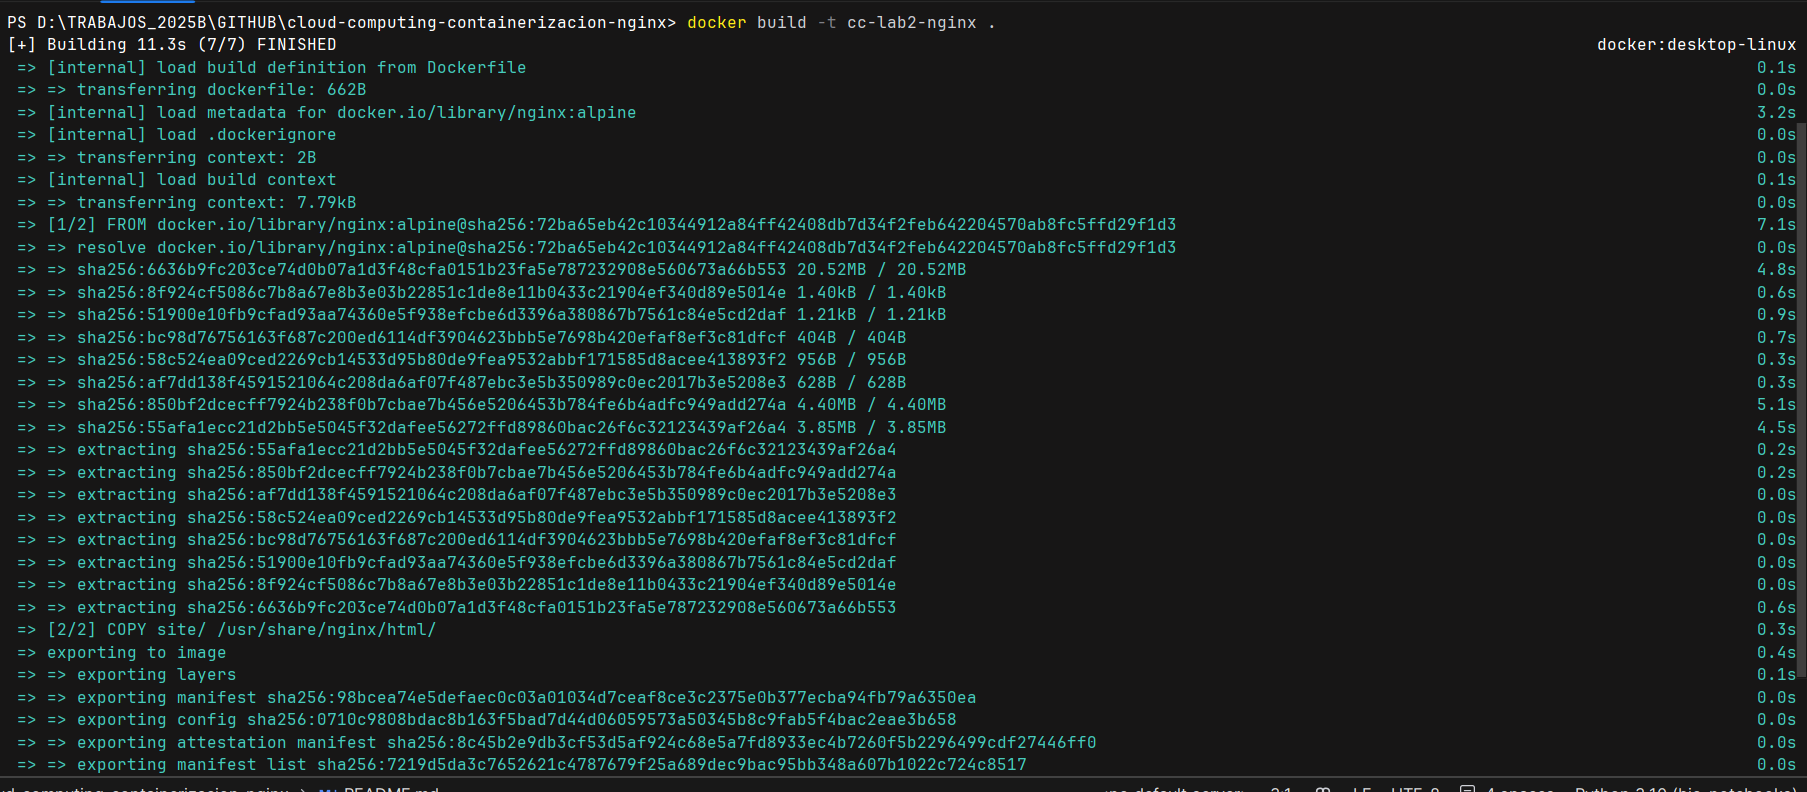
\includegraphics[width=0.85\textwidth]{figuras/evidencia1_build.png}
  \caption{Construcción exitosa de la imagen con \texttt{docker build}.}
  \label{fig:build}
\end{figure}

\subsection{Contenedor en ejecución}
\begin{figure}[h]
  \centering
  % 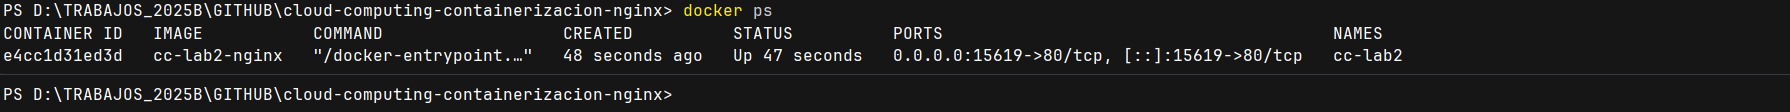
\includegraphics[width=0.85\textwidth]{figuras/evidencia2_docker_ps.png}
  \caption{Salida de \texttt{docker ps} mostrando el contenedor activo
  con el mapeo de puertos 15619→80.}
  \label{fig:ps}
\end{figure}

\subsection{Página accedida por el puerto 15619}
\begin{figure}[h]
  \centering
  % 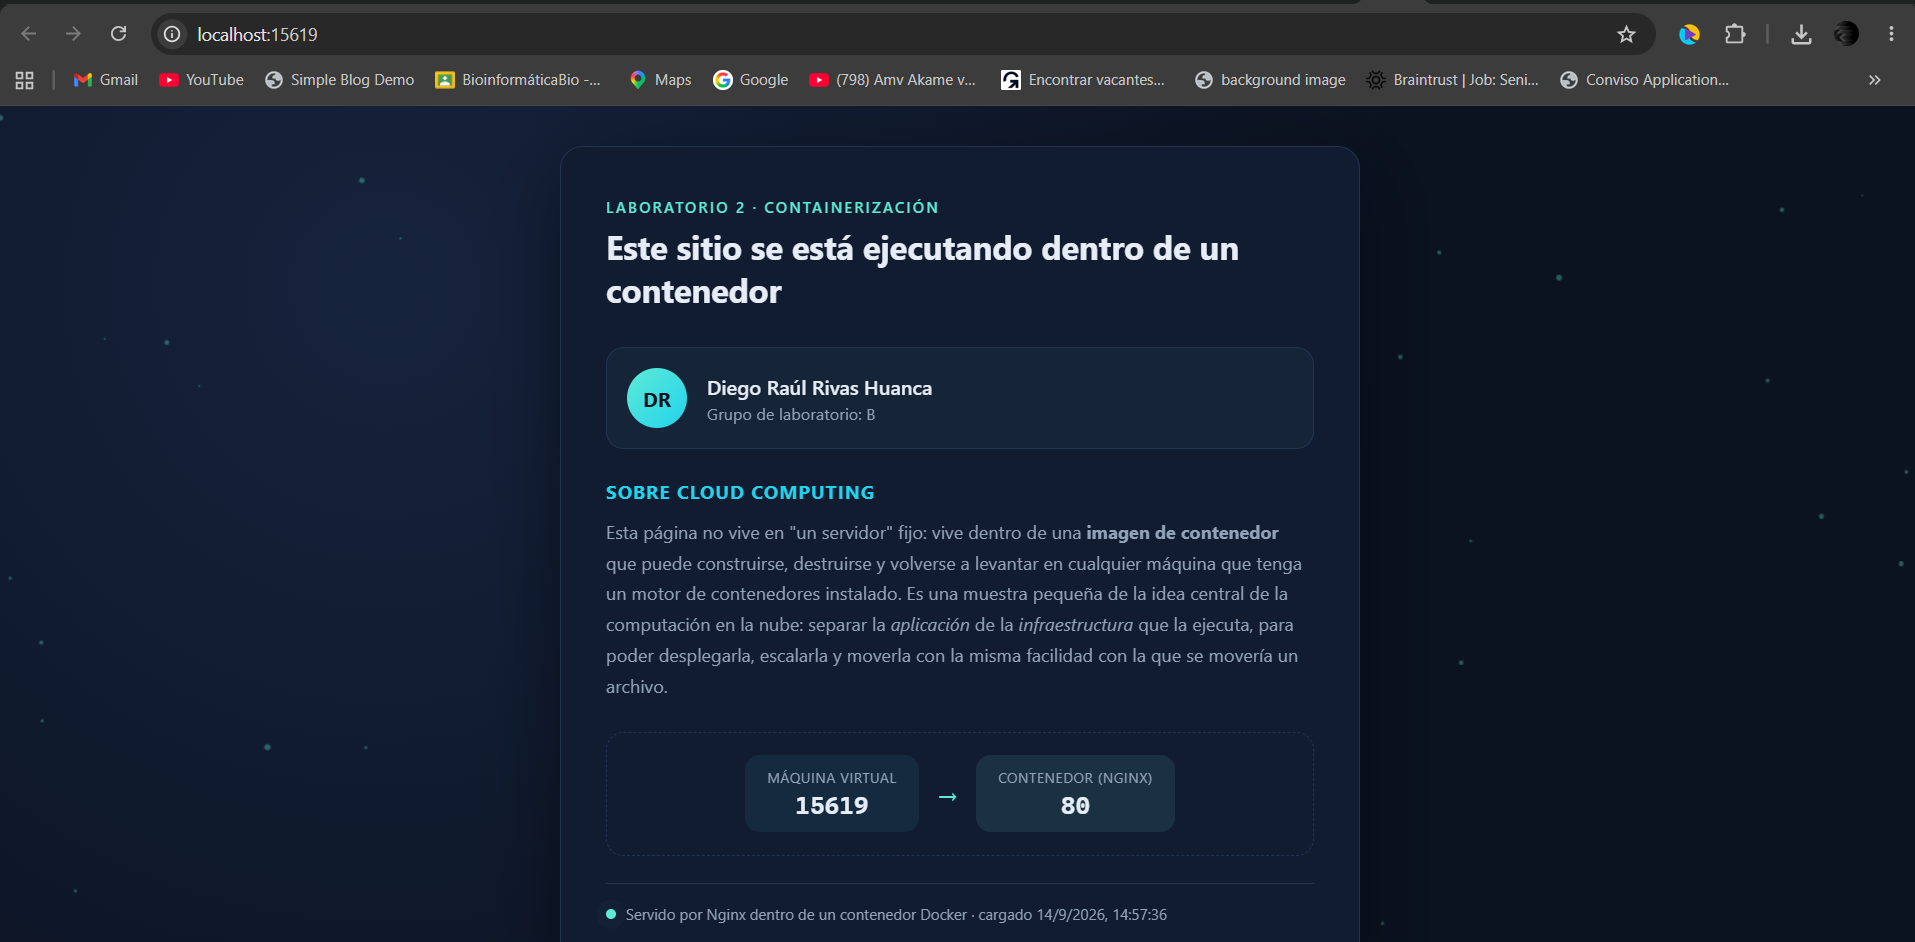
\includegraphics[width=0.85\textwidth]{figuras/evidencia3_navegador.png}
  \caption{Navegador mostrando la página personalizada en
  \texttt{http://localhost:15619}.}
  \label{fig:navegador}
\end{figure}

\subsection{Detención y nueva ejecución del contenedor}
\begin{figure}[h]
  \centering
  % 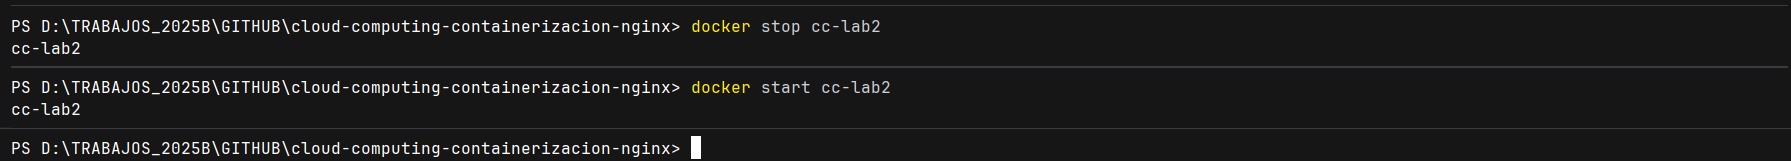
\includegraphics[width=0.85\textwidth]{figuras/evidencia4_stop_start.png}
  \caption{Secuencia \texttt{docker stop} seguida de \texttt{docker
  start} sobre el mismo contenedor.}
  \label{fig:stopstart}
\end{figure}

\textbf{Observación del requerimiento 10:} al ejecutar
\texttt{docker stop cc-lab2} el contenedor se detiene pero no se
elimina; \texttt{docker start cc-lab2} vuelve a levantar exactamente
el mismo contenedor (mismo ID, mismo filesystem) y la página vuelve a
estar disponible en el puerto 15619 sin necesidad de reconstruir la
imagen ni de repetir el flag \texttt{-p}, porque el mapeo de puertos
quedó fijado al crear el contenedor con \texttt{docker run}.

\section{Diferencia entre el puerto de la VM y el puerto del contenedor}
El puerto 80 es interno: es el puerto en el que Nginx escucha
\emph{dentro} del contenedor, aislado del resto del sistema. El puerto
15619 pertenece a la máquina virtual (el host) y es el que realmente
queda abierto hacia el exterior. El flag \texttt{-p 15619:80} crea un
reenvío (\emph{port forwarding}): todo lo que llega al puerto 15619 de
la VM se redirige al puerto 80 dentro del contenedor. Sin esa
publicación explícita, el puerto 80 del contenedor no sería alcanzable
desde fuera de él, aunque Nginx sí esté escuchando allí.

\section{Prompts de IA utilizados}
De acuerdo al punto 6 del enunciado, se listan a continuación los
prompts principales usados como apoyo para investigar sintaxis,
resolver errores y comprender las instrucciones de Docker (listado
completo también disponible en \texttt{prompts.md} del repositorio).

\begin{enumerate}
  \item Construcción de un Dockerfile para Nginx sirviendo una página
        HTML personalizada, y ubicación correcta del \texttt{COPY}.
  \item Diferencia entre \texttt{EXPOSE} y el flag \texttt{-p} al
        publicar puertos.
  \item Diferencia entre \texttt{docker stop}/\texttt{start} y
        \texttt{docker rm}/\texttt{run} de nuevo.
  \item Organización del proyecto en carpetas separadas para HTML,
        CSS y JS.
  \item Explicación conceptual, para el informe, de la diferencia
        entre el puerto de la VM y el puerto del contenedor.
\end{enumerate}

\section{Conclusión}
El laboratorio permitió comprobar de forma práctica cómo una misma
aplicación (la página web) puede empaquetarse en una imagen de
contenedor reproducible y ejecutarse de forma aislada, exponiendo
únicamente el puerto necesario hacia la máquina virtual. Se evidenció
además que detener y volver a levantar un contenedor no reconstruye la
imagen ni pierde su configuración de red, lo que ilustra la diferencia
entre el ciclo de vida de una \emph{imagen} y el de un
\emph{contenedor}.

\end{document}
